\documentclass[11pt]{report}
\usepackage{textcomp}

\usepackage{titlesec}
\titlespacing*{\section}
{0pt}{\baselineskip}{0em}
\titlespacing*{\subsection}
{0pt}{\baselineskip}{0em}

\usepackage{geometry}
\geometry{left=1in, right=1in, top=1in, textheight=9in}

\usepackage{enumitem}
\newlist{steps}{enumerate}{1}
\setlist[steps, 1]{wide=0pt, leftmargin=\parindent, label=Step \arabic*:}

\usepackage{fancyhdr}
\fancypagestyle{plain}{%
    \fancyhf{} % clear all header and footer fields
    \fancyfoot[C]{\sffamily\fontsize{.75em}{.75em}\selectfont\thepage} % except the center
    \renewcommand{\headrulewidth}{0pt}
    \renewcommand{\footrulewidth}{0pt}
}
\pagestyle{plain}

\usepackage{graphicx}
\graphicspath{ {./media/} }

\usepackage{setspace}
\doublespacing

\usepackage{minted}
\usepackage{xcolor}
\definecolor{LightGray}{gray}{0.9}
\newmintinline[asm]{asm}{fontsize=\small, bgcolor=LightGray}
\newmintinline[cpp]{cpp}{fontsize=\small, bgcolor=LightGray}

\AtEndEnvironment{listing}{\vspace{-1em}} % <-------

% make fancy title page
\makeatletter
\newcommand{\@labsection}{000}
\newcommand{\labsection}[1]{
    \renewcommand{\@labsection}{#1}
}

\newcommand{\@labnumber}{0}
\newcommand{\labnumber}[1]{
    \renewcommand{\@labnumber}{#1}
}

\newcommand{\@shortsubmitted}{1/1/70}
\newcommand{\shortsubmitted}[1]{
    \renewcommand{\@shortsubmitted}{#1}
}

\lfoot{\footnotesize \textit{University of Arkansas \\ EECS Department}}
\rfoot{\footnotesize \textsl{\@shortsubmitted}}

\renewcommand{\maketitle}{
    \newgeometry{left=1in, right=1in, top=1.75in, textheight=8.25in}
    \singlespacing
    \begin{center}
        {\huge \bf CSCE 22104} \\
        \vspace{2.5em}
        {\Large \bf Lab Report} \\
        \vspace{2em}
        \noindent\rule{20em}{0.4pt} \\
        \vspace{1em}
        {\Large \@author} \\
        \vspace{.75em}
        {\normalsize ID: 011019116} \\
        \vspace{.75em}
        {\normalsize Lab Section \@labsection} \\
        \vspace{.75em}
        {\normalsize Lab \@labnumber} \\
    \end{center}
    \newpage
    \restoregeometry
}

\makeatother


% TEXTWIDTH = 100
\begin{document}
\title{Lab Report 3}
\author{Brent Marcus Orlina}

\labsection{001}
\labnumber{3}

\shortsubmitted{3/7/25}

\maketitle

\section*{Introduction}
This lab's goal was to learn basic MIPS assembly by creating a basic program and translating two C++
programs, \verb|arrays.cpp| and \verb|occurence.cpp|, into MIPS assembly. The goal \verb|sum3.s| was
allow the user to input 3 integers and its sum. The \verb|arrays.cpp| program consisted of
initializing an array of integers and printing its elements. Finally, the \verb|occurences.cpp|
program consisted of allowing the user to input 10 integers into an array and another integer, $n$,
outputting the number of occurences of $n$ in the array.

\newpage

\section*{Approach}
\begin{listing}[h!]
    \inputminted[
        frame=lines,
        breaklines,
        linenos,
        tabsize=4,
        fontsize=\footnotesize,
        bgcolor=LightGray
    ]{asm}{./media/sum3-once.s}
    \caption{}
    \label{listing:sum3-once}
\end{listing}

For the \verb|sum3.s| program its goal is to read three integers from the user and output its sum to
the terminal. First, a prompt for the user to input an integer is first printed. This is done by
loading an opcode of \verb|4| into the register \verb|$v0| and loading the address of the string to
be printed into the register \verb|$a0|, using the instructions \verb|li| and \verb|la|
respectively. Then, the instruction \verb|syscall|, short for system call, is called which asks the
operating system to execute the given opcode in the register \verb|$v0| which in this case is to
print a string.

Similarly, the program uses another system call to read an integer from the user input. An opcode of
\verb|5| is loaded into the register \verb|$v0| and \verb|syscall| is called. After the user inputs
an integer, the operating system writes the given integer into register \verb|$v0|. This is moved
into a different register, in this case register \verb|$s0|, since \verb|$v0| will be used again for
more system calls.

The program has successfully read an integer from the user. To read the two other integers, the six
instructions shown in listing \ref{listing:sum3-once} is simply repeated two more times, with the
two new integers moved to registers \verb|$s1| and \verb|$s2| respectively.

\newpage

\begin{listing}[h!]
    \inputminted[
        frame=lines,
        breaklines,
        linenos,
        tabsize=4,
        fontsize=\footnotesize,
        bgcolor=LightGray
    ]{asm}{./media/sum3-addition.s}
    \label{listing:sum3-addition}
    \caption{}
\end{listing}

To calculate the sum of the three integers, the instruction \verb|add| is used. Since it is
impossible to add more than two integers at once in MIPS assembly (excluding the use of SIMD
instructions), the program must use two addition instructions, as shown in listing
\ref{listing:sum3-addition}. The program first adds the two integers in the registers \verb|$s0| and
\verb|$s1| and stores the result to register \verb|$t0|. Then, the program adds the result of the
first sum and the integer in \verb|$s2|, storing the result in register \verb|$s3|.

\begin{listing}[h!]
    \inputminted[
        frame=lines,
        breaklines,
        linenos,
        tabsize=4,
        fontsize=\footnotesize,
        bgcolor=LightGray
    ]{asm}{./media/sum3-print_output.s}
    \label{listing:sum3-print_output}
    \caption{}
\end{listing}

To output the sum of the three integers, a string is first printed, stating that the following
integer is the sum of the three given integers. The sum is then printed. This is done similarly
to printing the string \verb|input_prompt| earlier, with the exception that opcode \verb|1| is used
and the sum is moved from register \verb|$s3| to \verb|$a0| when printing the sum, as shown in
listing \ref{listing:sum3-print_output}.

\newpage

\begin{listing}[h!]
    \inputminted[
        frame=lines,
        breaklines,
        linenos,
        tabsize=4,
        fontsize=\footnotesize,
        bgcolor=LightGray
    ]{asm}{./media/sum3-exit.s}
    \label{listing:sum3-exit}
    \caption{}
\end{listing}

The program actually starts at the label \verb|_start|, which immediately jumps to the label
\verb|main|, as shown in listing \ref{listing:sum3-exit}. The \verb|jal| instruction jumps to the
given label, and saves the address it of the instruction after from where it jumped from in the
register \verb|$ra|. The program, after executing all of the instructions described previously,
jumps back to line 9 in listing \ref{listing:sum3-exit}, with the instruction \verb|jr|, so that the
program can properly exit using the correct syscall. The two translated C++ programs also exit
similarly as described. Describing the syscalls to read or print data will also be skipped since it
has already been described in this program and so that the attention can be focused on the
interesting parts of the implementation.

\begin{listing}[h!]
    \inputminted[
        frame=lines,
        breaklines,
        linenos,
        tabsize=4,
        fontsize=\footnotesize,
        bgcolor=LightGray
    ]{cpp}{./media/arrays.cpp}
    \label{listing:arrays-cpp}
    \caption{}
\end{listing}

Listing \ref{listing:arrays-cpp} shows the C++ program that was translated. The first part of the
program is printing a string \verb|"Numbers: "| followed by a newline. The second part of the
program is initializing an integer array with eight pre-defined values. The third part of the
program is that each integer in the array is printed followed by a newline using a for-loop.

\newpage

\begin{listing}[h!]
    \inputminted[
        frame=lines,
        breaklines,
        linenos,
        tabsize=4,
        fontsize=\footnotesize,
        bgcolor=LightGray
    ]{asm}{./media/arrays-init.s}
    \label{listing:arrays-init}
    \caption{}
\end{listing}

Listing \ref{listing:arrays-init} shows the implementation of the first two parts of the
\verb|arrays.cpp| program. Initializing the intger array \verb|x| in MIPS assembly was done by
declaring a label for the array in the \verb|.data| section and using the \verb|.word| directive to
indicate that the following sequence of data has the size of a word, 32-bits in the used
architecture.

\begin{listing}[h!]
    \inputminted[
        frame=lines,
        breaklines,
        linenos,
        tabsize=4,
        fontsize=\footnotesize,
        bgcolor=LightGray
    ]{asm}{./media/arrays-loop.s}
    \label{listing:arrays-loop}
    \caption{}
\end{listing}

\newpage

The for-loop can be broken down into four parts: intialization, conditions checking, main body,
incrementing. In listing \ref{listing:arrays-loop}, each part can be mapped explicitly.
Initialization occurs from lines 5 to 7. The variable \verb|i| is initialized to 0 in register
\verb|$s1|, which will be used to index into the integer array. The array size is initialized to
\verb|32| in register \verb|$s2|. The array size is 32 and not 8 since each element in the array is
4 bytes. Therefore it is initialize it to $8 \times 4 = 32$. Finally, the address of the array is
initialized to register \verb|$s0|.

The next part is checking the conditions of the loop to keep running. In listing
\ref{listing:arrays-cpp}, the condition is that the variable \verb|i| is less than \verb|8|, which
is the size of the array. That condition can be inverted so that if the condition is met, the loop
can exit and otherwise, the loop can keep running. This is shown in line 10 of listing
\ref{listing:arrays-loop} with the instruction \verb|bge| checking that the value in register
\verb|$s1| is greater than or equal to (the inversion of strictly less than) the value in register
\verb|$s2|. If the condition is met, the program jumps to the label \verb|loop_exit| in which case
the program exits. Otherwise, the loop continues to the main body of the loop.

The main body of the loop consists of printing the element at the current index. To do this, the
program must calculate the address of the element in memory and load it to a register as shown in
lines 12 and 13. This is done by adding the base address of the array and the current index and
using the result to load it into the register \verb|$t1|. Then, the element is printed along with a
new line. It is not shown in listing \ref{listing:arrays-loop} since it is trivial. However the
implementation can be seen in the appendix in listing \ref{listing:arrays-print}.

The final part of the loop increments the index, \verb|i|, by \verb|4| with the instruction
\verb|addi|. It is incremented by 4 since the elements are each 4 bytes in size. Thus, to get to the
next element, the program must skip every 4 bytes to get to the first byte of the next element.
After incrementing, the loop is ready to start over by jumping back to the \verb|loop_start| label
as shown on line 20. With the loop complete, the translation of the \verb|arrays.cpp| program is
completed.

\newpage

\begin{listing}[h!]
    \inputminted[
        frame=lines,
        breaklines,
        linenos,
        tabsize=4,
        fontsize=\footnotesize,
        bgcolor=LightGray
    ]{cpp}{./media/occurences.cpp}
    \label{listing:occurences-cpp}
    \caption{}
\end{listing}

Listing \ref{listing:occurences-cpp} shows the \verb|occurences.cpp| program to be translated. The
first part of the program is initializing the variables that the program will need. The second part
is printing an input prompt and reading ten integers from user input and storing them in an integer
array \verb|x|. Similarly, the third part is printing an input prompt and reading an integer from
user input storing it to the variable \verb|occur|. The fourth part is checking the number of times
that \verb|occur| is in the array \verb|x| and printing the indices that it is in. The final part is
printing the number of times that \verb|occur| is in, stored in the variable \verb|count|.

\begin{listing}[h!]
    \inputminted[
        frame=lines,
        breaklines,
        linenos,
        tabsize=4,
        fontsize=\footnotesize,
        bgcolor=LightGray
    ]{asm}{./media/occurences-init.s}
    \label{listing:occurences-init}
    \caption{}
\end{listing}

For the first part, only the strings and the array are needed to be initialized in the \verb|.data|
portion of the program since those live in memory while \verb|occur| and \verb|count| can simply
be initialized into registers once they are needed. The \verb|x_array| is initialized with the
\verb|.space| directive to signify that it should be empty with a size of \verb|40|, since there are
ten elements in the array, each the size of 4 bytes.

The second part of the program is trivial as it is extremely similar to the implementation the
translated \verb|arrays.cpp| program, with the only difference that it reads in an integer from user
input in the main body of the loop, and uses the store word instruction \verb|sw| instead of the
load word instruction \verb|lw|. The third part is also trivial since it is simply printing an
input prompt and reading an integer from user input, which is done in the \verb|sum3.s| program. The
implementations can be seen in the appendix, listings \ref{listing:occurences-sw} and
\ref{listing:occurences-occur}.

\begin{listing}[h!]
    \inputminted[
        frame=lines,
        breaklines,
        linenos,
        tabsize=4,
        fontsize=\footnotesize,
        bgcolor=LightGray
    ]{asm}{./media/occurences-loop.s}
    \label{listing:occurences-loop}
    \caption{}
\end{listing}

The fourth part is not as trivial as the loop contains an if-statement, however it is similar to
checking the conditions in a loop. Listing \ref{listing:occurences-loop} shows the loop that contains the if-statement.
It can be seen that it is extremely similar to the translation of the \verb|arrays.cpp| program, as
shown in listing \ref{listing:arrays-loop}. Note that the index, stored in register \verb|$s2|,
still increments by 4.

\newpage

\begin{listing}[h!]
    \inputminted[
        frame=lines,
        breaklines,
        linenos,
        tabsize=4,
        fontsize=\footnotesize,
        bgcolor=LightGray
    ]{asm}{./media/occurences-if.s}
    \label{listing:occurences-if}
    \caption{}
\end{listing}

Listing \ref{listing:occurences-if} shows the translation of the if-statement in listing
\ref{listing:occurences-cpp}. The if-statement can be broken into two parts: conditions checking,
and the main body. The condition for the if statement in listing \ref{listing:occurences-cpp} is
that if the current element is equal to \verb|occur|, then the main body can run. Otherwise, the
main body is skipped. Similar to conditions checking for for-loops, the condition can be inverted so
that if the inverted condition is met, the main body can be skipped. Otherwise, the main body runs.
Line 13 of listing \ref{listing:occurences-if} does this, by checking the value in register \verb|$s3|, the
variable \verb|occur|, is not equal to the value in register \verb|$t1|, the value in the current
index. If the condition is met, it jumps to the label \verb|occur_ifexit|, skipping the main body of
the if-statement, after the label \verb|occur_ifstart|, entirely.

If the condition is not met, then the main body runs, which prints the current index and increments
the variable \verb|count| in register \verb|$s4| on line 25. Note that the program is not simply
moving the index from register \verb|$s2| to register \verb|$a0| since it is still skipping by 4. To
output the correct looking index, it divides it by 4 by bit-shifting the index to the right by 2
with the instruction \verb|srl|. The final part is, again, trivial as it simply prints a string and
an integer. The implementation can be seen in the appendix in listing
\ref{listing:occurences-count}. With all parts complete, the translation for the
\verb|occurences.cpp| program is completed.


\section*{Experimentation}
The program \verb|sum3.s| was tested by using positive and negative integers as well as zero,
verifying that the output of the program was the correct sum of the three given integers. The
translation of the program \verb|arrays.cpp| was verified by simply observing that all the elements
in the array in the program were printed and in the correct order. The translation of the program
\verb|occurences.cpp| was verified by inputting ten integers, ensuring there were repeats, and
choosing the occurence value to be one of the repeating integers. Then it was observed if the
program outputted the correct indices and count of the chosen occurence value.

\section*{Results \& Discussion}
\begin{figure}[h!]
    \centering
    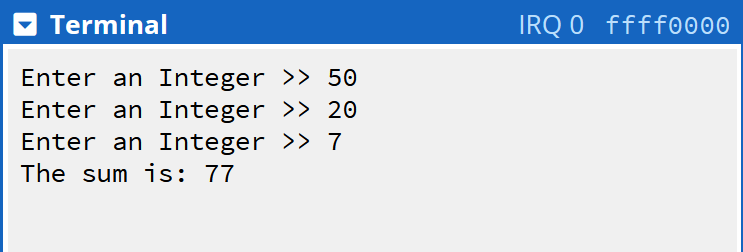
\includegraphics[width=0.9\textwidth]{sum3-terminal_positives}
    \label{fig:sum3-terminal_positives}
    \caption{}
\end{figure}

\begin{figure}[h!]
    \centering
    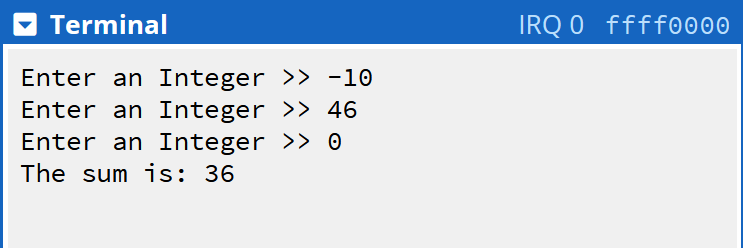
\includegraphics[width=0.9\textwidth]{sum3-terminal_negatives}
    \label{fig:sum3-terminal_negatives}
    \caption{}
\end{figure}

The program \verb|sum3.s| works as expected. Figures \ref{fig:sum3-terminal_positives} and
\ref{fig:sum3-terminal_negatives} shows the sums of three numbers. The first figure tests only
positive numbers while the second figure also tests negative numbers and a zero with each figure
showing the correct sums.

\newpage

\begin{figure}[h!]
    \centering
    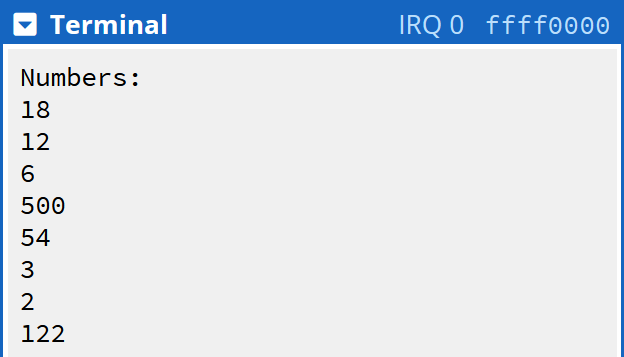
\includegraphics[width=0.6\textwidth]{arrays-terminal_output}
    \label{fig:arrays-terminal_output}
    \caption{}
\end{figure}

The translation of the program \verb|arrays.cpp| works as expected, with figure
\ref{fig:arrays-terminal_output} showing the translated program printing all the elements of the
array in the correct order.

\newpage

\begin{figure}[h!]
    \centering
    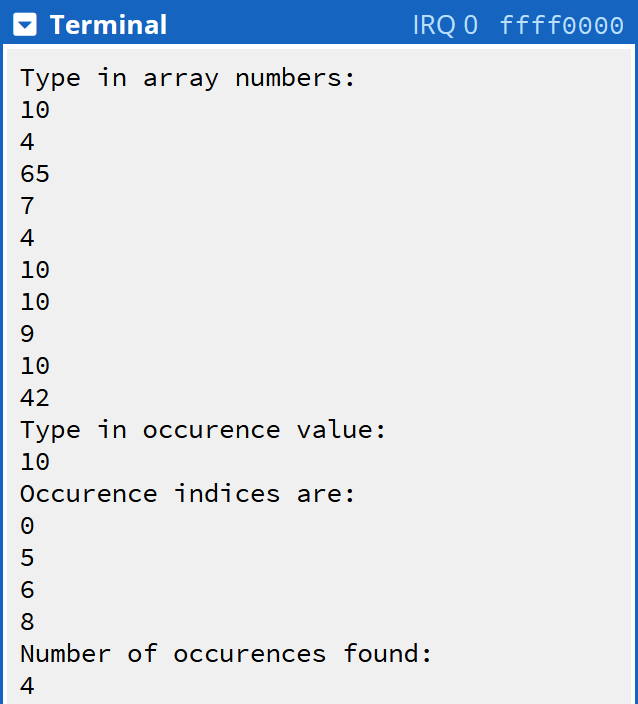
\includegraphics[width=0.6\textwidth]{occurences-terminal_output}
    \label{fig:occurences-terminal_output}
    \caption{}
\end{figure}

The translation of the program \verb|occurences.cpp| works as expected, with figure
\ref{fig:occurences-terminal_output} correctly printing the 0-indexed indices and the number of
occurences found of the user-given occurence value in the user-given integer array.


\section*{Conclusions}
The programs implemented in MIPS assembly in this lab works correctly. The knowledge learned from
implementing the \verb|sum3.s| program was reading user input, printing strings to the terminal,
initializing strings into memory, and adding integers inside of registers. In translating the
program \verb|arrays.cpp|, initializing arrays into memory, creating a for-loop, and indexing
into an array in MIPS assembly was learned. In translating the program \verb|occurences.cpp|,
creating an if-statement and writing into an array in MIPS assembly was learned.

% \newpage
% 
% \section*{References}
% \noindent
% [1]    Computer Organization 22104, EECS, University of Arkansas, “Lab 1,”  Sep. 17, 2024.
% 
% \noindent
% [2]    Computer Organization 22104, EECS, University of Arkansas, “Lab 2,”  Sep. 24, 2024.

\newpage

\section*{Appendix}
\begin{listing}[h!]
    \inputminted[
        frame=lines,
        breaklines,
        linenos,
        tabsize=4,
        fontsize=\footnotesize,
        bgcolor=LightGray
    ]{asm}{./media/arrays-print.s}
    \label{listing:arrays-print}
    \caption{}
\end{listing}

\newpage

\begin{listing}[h!]
    \inputminted[
        frame=lines,
        breaklines,
        linenos,
        tabsize=4,
        fontsize=\footnotesize,
        bgcolor=LightGray
    ]{asm}{./media/occurences-sw.s}
    \label{listing:occurences-sw}
    \caption{}
\end{listing}

\newpage

\begin{listing}[h!]
    \inputminted[
        frame=lines,
        breaklines,
        linenos,
        tabsize=4,
        fontsize=\footnotesize,
        bgcolor=LightGray
    ]{asm}{./media/occurences-occur.s}
    \label{listing:occurences-occur}
    \caption{}
\end{listing}

\newpage

\begin{listing}[h!]
    \inputminted[
        frame=lines,
        breaklines,
        linenos,
        tabsize=4,
        fontsize=\footnotesize,
        bgcolor=LightGray
    ]{asm}{./media/occurences-count.s}
    \label{listing:occurences-count}
\end{listing}

% \begin{figure}[h!]
%     \centering
%     \includegraphics[width=0.9\textwidth]{foo}
%     \label{fig:foo}
% \end{figure}
% 
% \newpage
% 
% \begin{figure}[h!]
%     \centering
%     \includegraphics[height=0.4\textheight]{bar}
%     
%     \label{fig:bar}
% \end{figure}
\end{document}
